\documentclass[fleqn,10pt]{olplainarticle}
% Use option lineno for line numbers 

\title{Proof of Concept II 
FOAR705 Digital Humanities}

\author{Roslyn Walker Student Number 45149631}
\keywords{ Existing platforms and systems: research photo tool, document management system, bibliography software.}
\begin{abstract}
Technology deployment computational analysis: virtual exhibition of visual content sourced from social media.
\end{abstract}
\begin{document}

\flushbottom
\maketitle

\section*{Computational Analysis}

Computational thinking is made up of four parts: 
\begin{enumerate}
\item Decomposition
\item Pattern recognition
\item Pattern generalisation and abstraction
\item Algorithm design

\end{enumerate}

\section{Decomposition}
In my Scoping Paper I, I identified the objective of the project is to build a repository for images online from social media that will form data for my thesis. Copyright management is in the scope of this project. The tasks include developing a dataset of images for cataloguing and adding contextual information about visual works in an archive collection (that is thematic tagging, making connections between objects, people, dates and places).

\section{Pattern recognition}
\begin{enumerate}
\item Capture material through thematic tagging to enable virtual exhibition display of content. I would like to curate these materials as a virtual exhibition.
\item Prepare a list of data types drafted as a tabular list in a word document and place this information into a spreadsheet format (Excel). The data types will be selected from standard usage terms of archive repositories. Description of images of other fields for the content records.
\item Output: Coding sheet of terms, Readme files, control vocabulary to make the task of tagging digital records easier when posting them to the repository as visual objects.
\item Data source files: Images sourced from social media hashtag publics on Instagram and Twitter.
\item Copyright restrictions on content may prevent the use of this material.
\item It would be great if I could automate the application of data tags and classification to the digitised record. I would like a tool that automatically applies tagging to the digital record.
\end{enumerate}

\section{Pattern generalisation and abstraction}
\begin{enumerate}
\item Initial setup format of data tables and resolve formatting issues for tabular data.
\item Source images and resolve copyright issues.
\item Discovery process for image use consider links or export options. 
\item Filter, sort and display of image and descriptive fields.
\end{enumerate}

\section {Algorithm Design}
\begin{enumerate}
\item Capturing material through thematic tagging to enable virtual exhibition display of content.
\item Images tagged in hashtag publics on social media platforms: FridaysForFuture YouthStrike4Climate ClimateEmergency GretaThunberg climatejustice ClimateStrike ExtinctionRebellion and ClimateHoax ClimateDenial
\end{enumerate}

\section*{Possible solutions}

Consideration to use a combination of the application of existing platforms and systems:
\begin{enumerate}
    \item https://tropy.org/ an example of a research photo tool to locate archival sources to write about them. 
\item Document management system (CMS or DMS)
\item Bibliography software like Zotero
\end{enumerate}

\section*{Some Examples of data sources}

\subsection*{Figures}

\begin{figure}[ht]
\centering
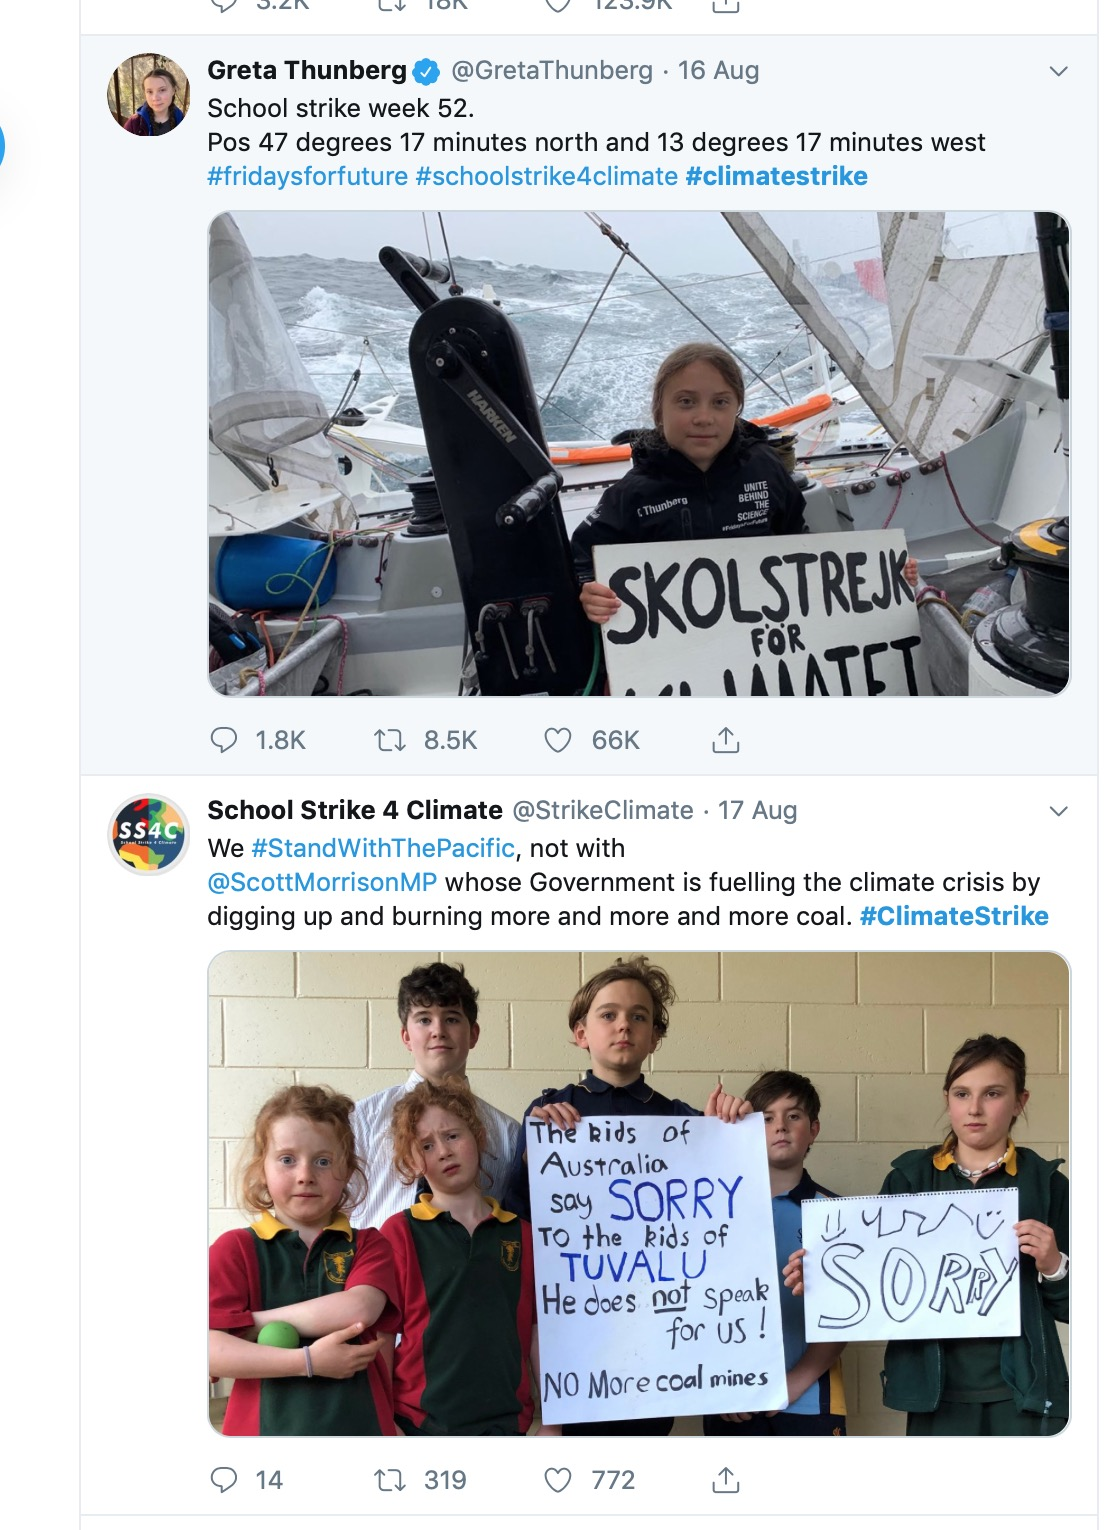
\includegraphics[width=0.5\linewidth]{Climatestrike_twitter}
\caption{Source: Twitter, ClimateStrike, 22 August 2019.}
\label{fig:view}
\end{figure}

\begin{figure}[ht]
\centering
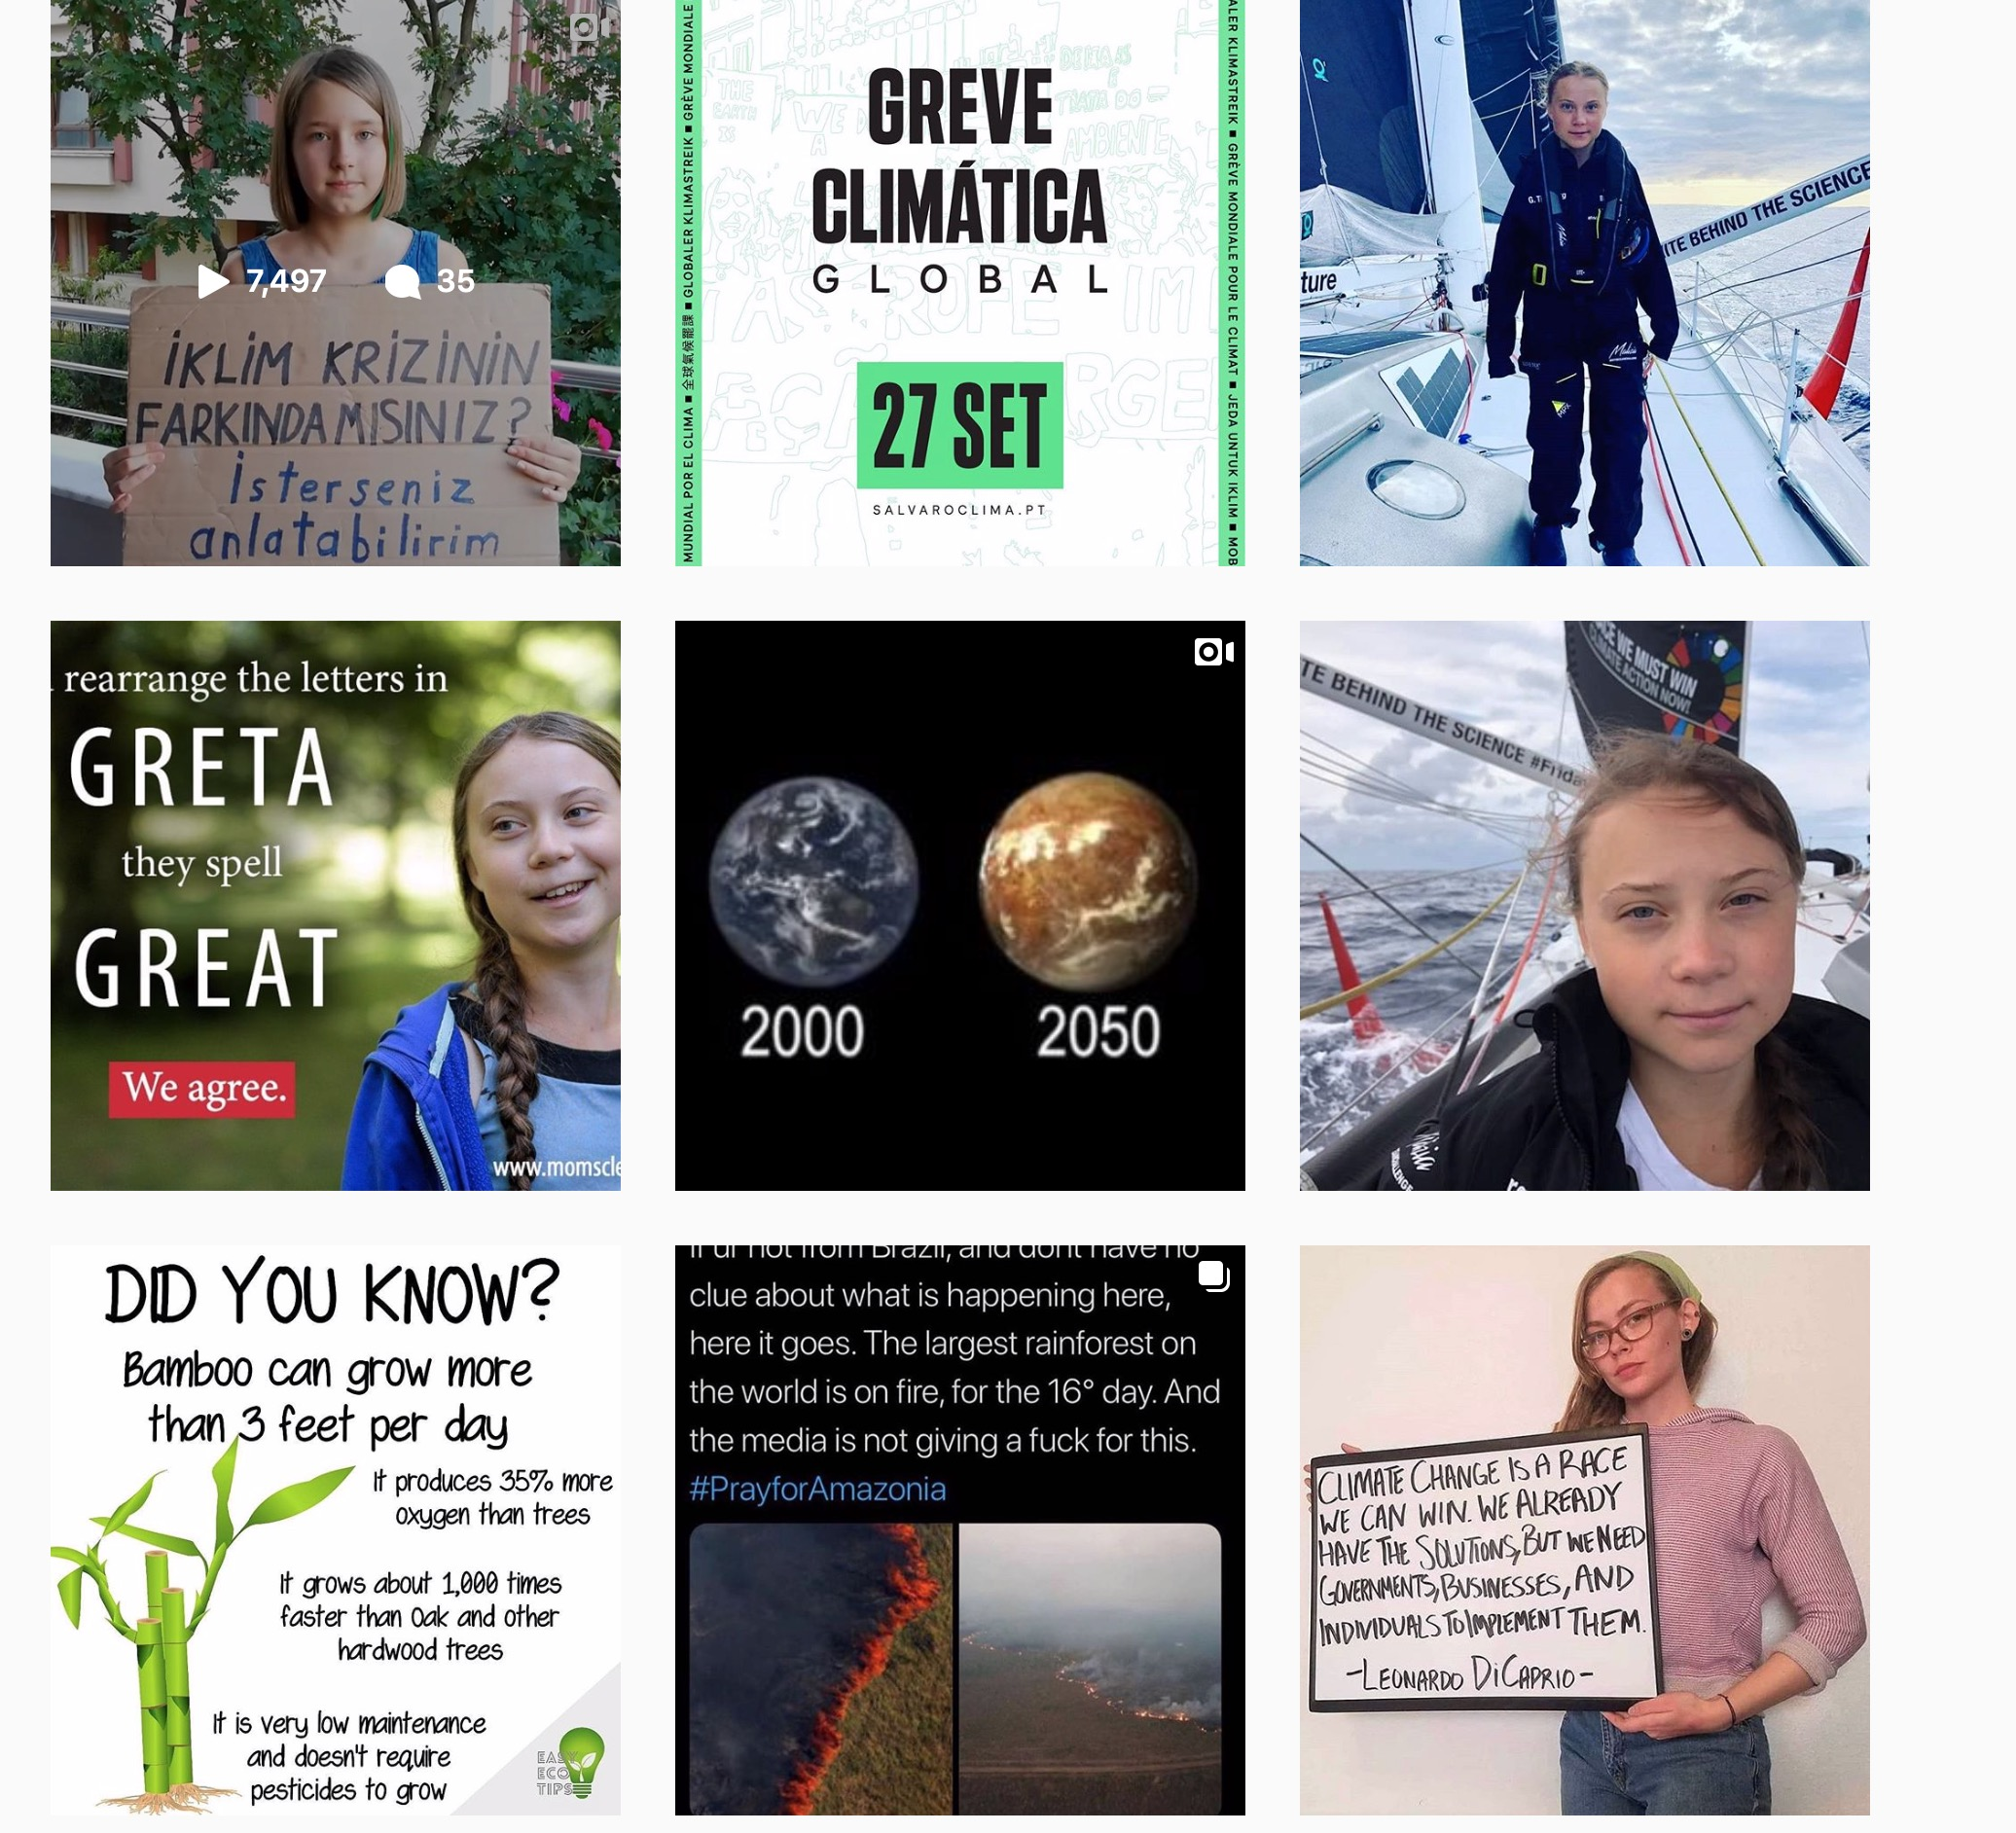
\includegraphics[width=0.5\linewidth]{Climatestrike_insta}
\caption{Source: Instagram, Schoolstrike4climate, 22 August 2019.}
\label{fig:view}
\end{figure}




\end{document}